% Dans l'introduction, on présente le problème étudié et les buts
% poursuivis. L'introduction permet de faire connaître le cadre de la
% recherche et d'en préciser le domaine d'application. Elle fournit
% les précisions nécessaires en ce qui concerne le contexte de
% réalisation de la recherche, l'approche envisagée, l'évolution de
% la réalisation. En fait, l'introduction présente au lecteur ce
% qu'il doit savoir pour comprendre la recherche et en connaître la
% portée.

\Chapter{INTRODUCTION}\label{sec:Introduction}  % 10-12 lignes pour introduire le sujet.

\\
Support d'acrobatie, entrainant le corps de l'utilisateur qui s'y accroche dans un mouvement de rotation, mais pouvant aussi bien être manipulée par ce dernier, la roue Cyr se place à mi-chemin entre les disciplines acrobatiques, les disciplines d'équilibrisme et la manipulation d'objet. La réalisation de figures acrobatiques repose sur un équiibre dynamique continuel entre la roue et le corps de l'utilisateur: ce dernier influe sur le mouvement de la roue, tout en modulant le rythme et la force qu'il applique en fonction des caractéristiques de la roue (sa masse, son inertie, sa géométrie). Un changement dans ces caractéristiques rend ainsi nécessaire l'adaptation de l'artiste à une variation du mouvement. La popularité croissante de l'utilisation de matériaux composites pour la fabrication d'équipement de cirque comme les mats ou les portiques éveille l'intérêt de la communauté circassienne sur les possibilités nouvelles qu'une roue Cyr faite d'un tel matériau peut apporter. L'enjeu est double: le procédé de fabrication offrant un éventail de possibilités géométriques inaccessibles avec les métaux ainsi qu'un choix des propriétés mécaniques beaucoup plus large, on y voit une occasion d'optimiser les mouvements déjà existants mais aussi d'inventer de nouvelles figures avec une roue Cyr faite d'un matériau dont les propriétés élastiques permettent, par exemple, de sauter avec la roue.
%%
%%  CONCEPTS DE BASE / BASIC CONCEPTS
%%
\section{Définitions et concepts de base}  % environ 2-3 pages



\subsection{Définitions}
\paragraph{Circassien(ne):} relatif au cirque 
\paragraph{Agrès de cirque:} équipement nécessaire à la pratique d'une discipline circassienne. Exemples: la roue Cyr, le trapèze, le tissu aérien, les cannes d'équilibre, le mat chinois...
\paragraph{Disque d'Euler:} disque ayant un mouvement de rotation similaire à celui d'une pièce qu'on fait tourner sur une surface plane. Lorsque son mouvement entre en phase terminale sa vitesse de rotation augmente de façon impressionnante, ce qui lui a valu de devenir un jouet éducatif, mais aussi de faire l'objet de nombreuses publications scientifiques. Son mouvement est similaire à un des mouvements caractéristiques de la roue Cyr.


\subsection{Historique de la roue Cyr}
La roue Cyr que l'on retrouve dans les spectacles de cirque contemporains doit son  nom à Daniel Cyr, qui fabriqua sa première roue en 1996 \cite{Inertie}. A cette dernière, faite en une seule pièce d'acier recouverte d'un revêtement en PVC afin d'améliorer l'adhérence avec le sol, succéda rapidement  une roue Cyr démontable en plusieurs parties. La première apparition marquante de la roue Cyr sur la scène circassienne eut lieu en 1998 dans un spectacle du Cirque Eloize, dont Daniel Cyr est le co-fondateur. Une médaille d'argent remportée en 2003 par ce dernier au Festival Mondial du Cirque de Demain acheva d'assoir la popularité de ce nouvel agrès dans le secteur du cirque, mais également en tant que sport.\\
Cependant l'idée d'une roue à la géométrie torique dont le diamètre avoisine la taille humaine remonte bien avant la création de Daniel Cyr \cite{Inertiehist,gymmedia,howstuffwork}. En effet, plusieurs agrès d'apparence similaire à celle de la roue Cyr ont fait leur apparition du côté de l'Allemagne dès le début du vingtième siècle. On remarquera en particulier l'Einrefen, inventé en 1930 par Adalbert von Rekowski, qui diffère de la roue Cyr par des poignées intérieures pour les mains et les pieds. \\
Depuis, la roue Cyr continue d'évoluer, comme le montrent les agrès dérivés présentés à la fin du manuel de la FEDEC (Fédération Européenne Des Ecoles de Cirque professionnelles) \cite{Fedec2011}. Les procédés de fabrication se sont eux aussi affinés \cite{corbin}, et les roues Cyr lumieuses programmables ont vu le jour.\\
La fabrication en matériaux composites se présente aujourd'hui comme l'étape suivante dans l'évolution de l'agrès.

\subsection{Les figures de roue Cyr}
Nous présentons ici les figures de roue Cyr constituant la base principale de la discipline. Ces dernières, ainsi que d'autres figures plus approfondies sont détaillées dans le manuel de la FEDEC \cite{Fedec2011}
\subsubsection{La valse (ou pas de base)}
Le corps est positionné de façon symétrique, avec bras et jambes chacun inclinés à 45\degree de la verticale. L'utilisateur initie la rotation d'une poussée du pied puis accompagne le mouvement de la roue en utilisant le tranfert de son poids, tirant et poussant successivement la roue dans le sens de la rotation.\\
Ce mouvement se décline en plusieurs variations en ajoutant par exemple un lacher de pieds, qui avec un arc de cercle de la jambe devient un arabesque, ou encore en l'exécutant à une seule main ou mains croisées, en serrant et croisant les jambes ou en les écartant jusqu'au grand écart latéral. Cette figure s'exécute aussi avec un pied placé sur la roue au niveau de la tête, en grand écart facial. On peut aussi varier en jouant avec la position du corps: corps de profil, dans le plan de la roue, arqué vers l'intérieur, tendu vers l'extérieur...

\subsubsection{Les tours}
Dissociation du mouvement: la roue tourne mais pas le corps. Ce type de figure peut être exécuté en effectuant un demi-tour, un tour complet, ou même un tour en suspension avec l'utilisateur suspendu à la roue par une main.

\subsubsection{Les vrilles}
Dissociation inverse, le corps tourne dans le reférentiel de la roue. De même ce type de figure se décline en diverses sortes de demi vrilles et en vrille complète en suspension.

\subsubsection{Les suspensions}
Comme l'indique le nom, les pieds ne sont pas sur la roue. On peut par exemple exécuter la valse en suspension, sans les pieds, ou simplement prendre de l'élan puis lacher les pieds et adopter une position groupée en tournant sur place, ce qui a pour effet d'augmenter la vitesse de rotation. Il est possible de se suspendre par une ou deux mains, par les coudes, les bras tendus ou fléchis. La suspension est la base de la figure du Superman: corps gainé, jambes tendues vers l'extérieur de la roue.

\subsubsection{Le drapeau}
La roue n'est tenue que par la main et le pied d'un même côté. La rotation est alimentée en poussant et tirant avec la main et le pied restant, tout en tendant puis groupant successivement la main et le pied lachés.

\subsubsection{Les sauts}
La roue tourne sur elle même, l'utilisateur saute et prend appui come il le souhaite, bras tendus, pliés, ou même en position assise sur la roue. Il peut ensuite atterrir sur le sol ou directement sur la roue.

\subsubsection{Le corner ou inclinaison horizontale}
L'utilisateur se décale sur un côté de la roue jambes serrées, prend appui jambes fléchies puis plonge vers le sol, jambes tendues le corps se retrouve en position horizontale pour un demi tour. Cette figure peut se réaliser en lachant un bras, un pied, ou un bras et un pied simultanément.

\subsubsection{Le saut de mains}
L'utilisateur pousse la roue vers le sol avec une main, accompagne le renversement avec son poids, ouvre les doigts quand sa main arrive au niveau du sol puis la tire au dessus de sa tête et la pousse avec ses jambes afin de revenir à l'endroit. Cette figure s'exécute en avant, en arrière, en position de profil, à une jambe.

\subsubsection{La roue}
L'utilisateur exécute une roue classique tout en étant dans la roue au moyen de transferts de poids. Il est possible de réaliser cette figure en enchainant plusieurs roues le long d'une trajectoire circulaire, ou bien d'une ligne droite. Il est possible de la combiner avec d'autres figures et changements de directions et d'enchainer ainsi plusieurs roues dans des sens différents.

\subsubsection{La pièce}
Ce mouvement est semblable à la rotation d'une pièce de monnaie (ou du disque d'Euler) dans la phase terminale du mouvement. L'utilisateur, gainé, ouvre sucessivement les doigts pour ne pas les écraser lorsque ses mains arrivent au niveau du sol, et transfere son poids pour accompagner le mouvement et l'alimenter aussi longtemps qu'il le souhaite. Cette figure peut s'exécuter à différentes hauteurs du sol, plus la pièce est basse, plus la vitesse sera élevée. On peut aussi la réaliser à l'envers, le corps arqué (pièce dorsale).

\clearpage

%%
%lt% anément eELEMENTt chent la roue simuS DE LA PROBLEMATIQUE
%%
\section{Problématique}  % environ 3 pages
La création d'une roue Cyr en matériaux composites, aux propriétés différentes de celles qui roues Cyr métalliques, qui permettra d'enrichir la discipline de nouvelles figures se trouve au carrefour de la science, de la technique acrobatique et de l'art. Ceci nécessite de réunir des expertises issues de ces différents domaines, couplés à des moyens de fabrication adéquats. La problématique peut donc se découper selon les trois étapes caractéristiques du projet.

\subsection{Conception}
Il s'agit de déterminer quels paramètres parmi les propriétés mécaniques du matériau et la géométrie de la roue Cyr influencent de manière notable les mouvements de cette dernière, puis de caractériser cette influence quantitativement. \\ 
A cet effet des modèles théoriques de deux mouvements caractéristiques ont été développés:
\begin{itemize}
    \item Le saut (la possibilité d’intégrer des sauts aux figures de roue Cyr déjà existante étant une des lignes directrices du projet): la roue est compressée par l'exercice d'une force dont l’axe coincide avec le diamètre, puis relâchée. Une part de l’énergie élastique stockée est convertie en saut. 
    \item Le mouvement correspondant à celui d’une pièce de monnaie qui roule sur sa tranche en décrivant des cercles, puis entre en phase terminale avant de tomber à plat sur le sol.
\end{itemize}

En se basant sur chacun des modèles théoriques correspondants, l’objectif est de déterminer séparément les paramètres géométriques et mécaniques qui :
\begin{itemize}
    \item  permettent à l’utilisateur de sauter le plus haut possible avec la roue.
    \item permettent d’optimiser le mouvement similaire à celui de la pièce de monnaie décrit ci-dessus en termes de stabilité dynamique.
    \item conduisent au meilleur compromis entre les deux réponses aux questions précédentes.
\end{itemize}


Parallèlement, il est indispensable d’étudier les contraintes et déformations dans la roue et plus particulièrement celles dues à l’impact avec le sol lors des sauts afin d’identifier des zones de design, qui garantissent que cette dernière ne sera pas endommagée.

\subsection{Fabrication}
Il s’agit de compléter l’étude théorique issue de la phase de conception par une utilisation adaptée de l’impression 3D. En utilisant les technologies existantes et disponibles pour le projet, comment imprimer un tore d’un diamètre avoisinant les deux mètres ? Comment assurer des propriétés conformes à celles déterminées par les modèles théoriques établis au préalable ? 

\begin{figure}[htb]
\centering
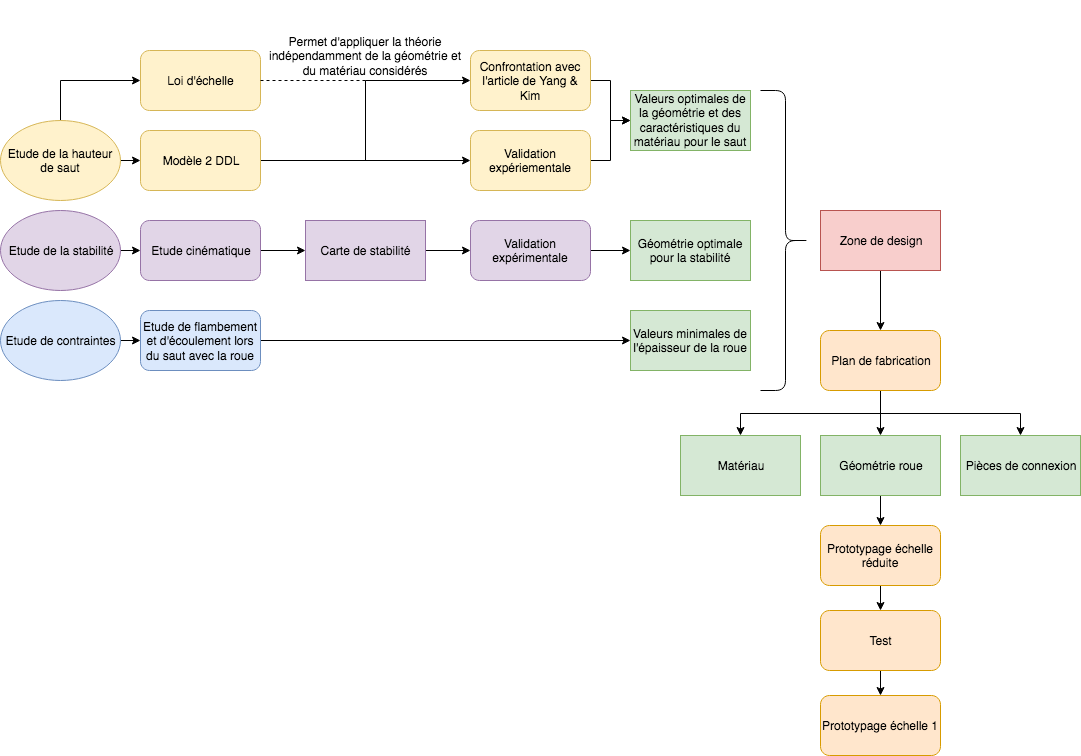
\includegraphics[width=7in]{images_autres/flowchart.png}
\caption{Flowchart résumant les étapes de conception et de fabrication de la roue.}
\label{fig:flowchart}
\end{figure}

\subsection{Tests}
Malgré la popularité du sujet au sein de la communauté circassienne et des pratiquants de roue Cyr, la roue en matériaux composites ne figure pas parmi les offres des fabricants d’équipement de cirque. Ces dernières sont en partie influencées par le fait qu’il y ait un flou, une difficulté à estimer concrètement ce qu’apporterait une telle roue Cyr et donc si les individus adeptes de la discipline seraient prêts à acquérir une roue Cyr composite, pour un prix bien supérieur à ceux des roues métalliques. En effet, leur fabrication nécessite un investissement conséquent qui ne peut être fait sans avoir de certitude sur sa rentabilité. Une phase de recherche artistique menée avec le prototype à l’échelle 1 imprimé et fonctionnel et en collaboration avec des artistes de roue Cyr de haut niveau, permettra de lever le voile sur les nouvelles possibilités introduites par une roue Cyr composite, aussi bien en termes d'acrobaties que de jeu de scène, ainsi que sur la réaction de la communauté et des pratiquants, ce qui permettra aux fabricants d'évaluer plus clairement si une véritable demande peut exister.\\
En outre, plusieurs artistes de roue Cyr ont déjà tenté d'approcher ces nouvelles possibilités, avec des roues Cyr fabriquées de manière artisanales dans des matériaux plus légers ou plus flexibles (par exemple une roue Cyr en osier a été fabriquée par des élèves au Centre National des Arts du Cirque (CNAC) en France)
cependant ces projets d'expérimentation n'ont pu être menés à terme, les roues se retrouvant rapidement endommagées et hors service. Ceci s'explique par le manque de moyens et de temps à consacrer à une étude préalable méthodique et approfondie rassemblant des expertises diverses et des moyens de fabrication adéquats, ainsi qu'une maitrise des procédés de fabrication additive. Fournir un prototype fonctionnel et solide permettra à ces artistes de continuer et d'approfondir leur recherche dans la sécurité, au terme de quoi la discipline pourrait prendre un nouveau tournant.\\


% On veut éviter que la figure et le tableau soient placés au-delà de la section courante.
\FloatBarrier


%%
%% OBJECTIFS DE RECHERCHE / RESEARCH OBJECTIVES
%%
\section{Objectifs de recherche}  % 0.5 page
\subsection{Objectif global}
L'objectif global de ce projet de recherche est de parvenir à la conception d’un prototype de roue Cyr haute performance aux propriétés élastiques, imprimé en 3D à partir d’un matériau optimisé, puis tester avec des artistes de haut niveau les nouvelles possibilités offertes par cet agrès

\subsection{Objectifs spécifiques}
Les objectifs spécifiques du projet sont les suivants:
\begin{itemize}
    \item Caractériser expérimentalement et théoriquement l’influence des propriétés mécaniques et des paramètres géométriques sur le comportement dynamique de la roue Cyr
    \item Développer un modèle numérique de la dynamique de la roue Cyr
    \item Définir un matériau composite haute performance optimisé pour la roue Cyr
    \item Imprimer un prototype en 3D à partir de ce matériau
    \item Conclure le projet par des sessions de recherche artistique autour du nouvel agrès
\end{itemize}


%%
%% PLAN DU MEMOIRE / THESIS OUTLINE
%%
\section{Plan du mémoire}  % 0.5 page
Ce mémoire s'organise en six chapitres. Le deuxième chapitre est constitué d'une revue de littérature centrée sur la roue Cyr, recensant les publications ayant pour objet des systèmes s'en rapprochant par leurs formes et leurs mouvements, tels que le disque d'Euler ou les anneaux élastiques. Le chapitre trois expose les modèles théoriques développés dans le but de répondre à la problématique exposée à l'introduction, leur implémentation numérique et les résultats et conclusions ainsi apportés. Il s'ensuit un quatrième chapitre présentant la méthodologie mise en oeuvre pour valider expérimentalement ces modèles, à l'aide de systèmes de taille réduite, mais aussi et surtout grace au prototype imprimé à l'échelle 1. Le cinquième chapitre présente les résultats de ces expériences et leur analyse. Le tout sera naturellement clôturé d'une conclusion.